\documentclass[../notes.tex]{subfiles}

\pagestyle{main}
\renewcommand{\chaptermark}[1]{\markboth{\chaptername\ \thechapter\ (#1)}{}}

\begin{document}




\chapter{???}
\section{Experimental Physical Chemistry: An Introduction}
\begin{itemize}
    \item \marginnote{1/3:}Questions:
    \begin{itemize}
        \item Is "Introduction to Nanotechnology by Linsay" the same as "Introduction to Nanoscience by Stuart M. Lindsay?"
        \begin{itemize}
            \item They'll check on this.
        \end{itemize}
        \item Access to Panopto recordings?
        \begin{itemize}
            \item I have access now.
        \end{itemize}
        \item Recordings of class content?
        \begin{itemize}
            \item Yes, if they can get the AV working.
        \end{itemize}
    \end{itemize}
    \item Intro by Hannah Lant (instructional professor to manage lab meetings). Tokmakoff handles lectures/non-in-lab stuff.
    \item Goals of the course.
    \begin{itemize}
        \item Demonstrate and interrogate principles from your theory courses, e.g., from QMech/Thermo.
        \item Learn practical techniques to characterize chemical and physical properties of molecules and nanomaterials, and the related spectroscopic techniques.
        \item Analysis of data (in-class and in-lab).
        \item What have you learned, and how can you communicate your findings to a scientific audience.
    \end{itemize}
    \item Everything helps everything else; it's cyclical from experimental theory, to collecting data, to data analysis, to communication, and back to more theory.
    \item Lectures will be more like workshops/recitations. There are recordings for content.
    \item Rest of today: Logistics and individual experiments.
    \item Canvas page.
    \begin{itemize}
        \item Syllabus.
        \item Most info on the Modules page.
        \item Fitting exercises will be in in-class meetings in the day to come.
        \item Experiments.
        \item Video lectures on Panopto.
    \end{itemize}
    \item Watch the 15-min Lecture 1 before class on Thursday!
    \item 6/9 weeks in lab. Complete a total of 6 experiments.
    \begin{itemize}
        \item Core experiments for weeks 2, 4-6 (UV/Vis, FT-IR, NMR, GC-MS).
        \begin{itemize}
            \item Full lab report on one of these; short lab report on the other ones.
        \end{itemize}
        \item Choose your experiments for weeks 7-8.
        \begin{itemize}
            \item Highlight content in nanomaterials and kinetics.
            \item Week 7 requires a full lab report on that experiment.
            \item Week 8 requires a group presentation on your experiment.
            \item Survey to determine what you do before Friday of Week 2!
        \end{itemize}
    \end{itemize}
    \item Grading breakdown.
    \begin{itemize}
        \item Prelab quizzes: 15\% (2.5\% per quiz).
        \begin{itemize}
            \item About 5 questions.
            \item Must get 80\% or above to attend lab.
            \item 2 attempts.
            \item Focus on safety, but also thinking critically about the theory for the lab.
        \end{itemize}
        \item Short reports: 40\% (10\% per report).
        \begin{itemize}
            \item How to do info --- in the lab manual.
            \item ACS citation style.
            \item There will be rubrics posted on Canvas (grading is not subject to the whims of our TAs).
        \end{itemize}
        \item Full reports: 30\% (15\% per report).
        \item Group oral presentation: 15\%.
        \begin{itemize}
            \item Attend a few other presentations and give ours during finals week.
        \end{itemize}
    \end{itemize}
    \item A full schedule of assignments and labs is available in the syllabus.
    \item See announcement for which lab cohort I'm supposed to be in!
    \item What the experiments are and what their purposes are (nontechnical because we haven't done the theory yet).
    \item Weeks 2, 4-6.
    \begin{itemize}
        \item UV/Vis to get a vibronic spectrum of iodine (to get electronic/vibrational data on \ce{I2}).
        \item FT-IR: Rovibrational information on \ce{HCl}.
        \item NMR: \ce{C5H11OH}.
        \item GC-MS: Separation science and MS. Analyze gasoline, which is a complex mixture of organic molecules.
    \end{itemize}
    \item Week 7 (+ info on who should choose these; think about it next week after first lab).
    \begin{itemize}
        \item Fluor: Fluorescence spectra of analytes, including pyrene.
        \begin{itemize}
            \item Both spectroscopy and kinetics. If you're really interested in physical chemistry and kinetics, do this. Uses custom built stuff in the labs.
        \end{itemize}
        \item QDots: Cadmium and Selenium nanocrystals.
        \begin{itemize}
            \item Applications of particle-in-a-box ideas, nanotechnology, synthesis, the prettiest one.
        \end{itemize}
        \item EChem: Developed by Anna Wuttig.
        \begin{itemize}
            \item More training in CV. Look at a number of different electrodes, and assay their activity in the hydrogen-evolution reaction. Applications in renewable energy.
            \item Will run both weeks 7-8.
            \item Includes some interaction with Wuttig.
        \end{itemize}
        \item AFM: Atomic force microscopy.
        \begin{itemize}
            \item Imaging a number of different materials, e.g., the grooves on a DVD. Great for anyone interested in nanoscience.
        \end{itemize}
    \end{itemize}
    \item Week 8:
    \begin{itemize}
        \item Photo: Alternate addition this week.
        \begin{itemize}
            \item Photodissociation of \ce{CO} from that hemoglobin structure and then some kinetics.
        \end{itemize}
    \end{itemize}
    \item The PChem lab suite: Enter Jones laboratory and turn left. We'll go elsewhere for special instrumentation. Lant's office is next door.
    \item NMR and GC-MS in Searle 340 instrumentation center. Usually meet our TA in the PChem lab suite and then travel.
    \item Attendance.
    \begin{itemize}
        \item You are required to attend all six lab sessions and record your own data (often in groups).
        \item Excused absences include university travel, family emergencies, and illness; please be in touch with Prof. Lant as soon as possible to reschedule your lab.
        \item Unexcused absences may be able to reschedule at a 20\% penalty if availability allows (this is an overenrolled class).
    \end{itemize}
    \item Safety.
    \begin{itemize}
        \item General lab safety policies from Gen Chem and OChem still apply.
        \item Bring your own goggles.
        \item Acknowledge you've reviewed the polices on Canvas in the first lab quiz.
        \item Safety tour of the lab space on your first lab day by your TA.
        \item Lab aprons will be provided.
        \item Specific safety concerns will be communicated in lab manuals and pre-lab quizzes.
    \end{itemize}
    \item We're all coming in with diverse scientific experiences. Fill out a survey on Canvas $>$ Assignments $>$ surveys or at \href{https://www.tinyurl.com/pchemlabsurvey}{tinyurl.com/pchemlabsurvey}!
    \item No formal lecture on Thursday in this room! There will be a series of about 7 video lectures over the first two weeks that cover what we need to know for our first core experiments (watch these!). Workshops during this period, too. E.g., if they find from the surveys that we don't have experience with fitting data very well, we'll work through that. There is an exercise for this on Canvas?? (Data Fitting Exercises.pdf explains it.)
    \item Tokmakoff puts a big emphasis on communication :)
    \begin{itemize}
        \item "Any professional science is communicated; otherwise, it's just a hobby."
        \item Should be nicely formatted with good figures, etc.
    \end{itemize}
    \item My lab group: Thursday A.
    \item Schedule.
    \begin{itemize}
        \item UV/Vis: 1/12.
        \item FT-IR: 1/26.
        \item NMR: 2/2.
        \item GC-MS: 2/9.
    \end{itemize}
\end{itemize}



\section{Lecture 1: Principles of Spectroscopy}
\begin{itemize}
    \item \textbf{Spectroscopy}: Studying the properties of matter (e.g., molecules and materials) through its interaction with different frequency components of the electromagnetic spectrum. \emph{Etymology} \textbf{spectron} from Latin "ghost" or "spirit."
    \begin{itemize}
        \item More on the etymology: An apt description because you never see the molecule itself; you see a representation/image/apparition of it.
    \end{itemize}
    \item Each type of spectroscopy gives a different picture (the \emph{spectrum}).
    \begin{figure}[h!]
        \centering
        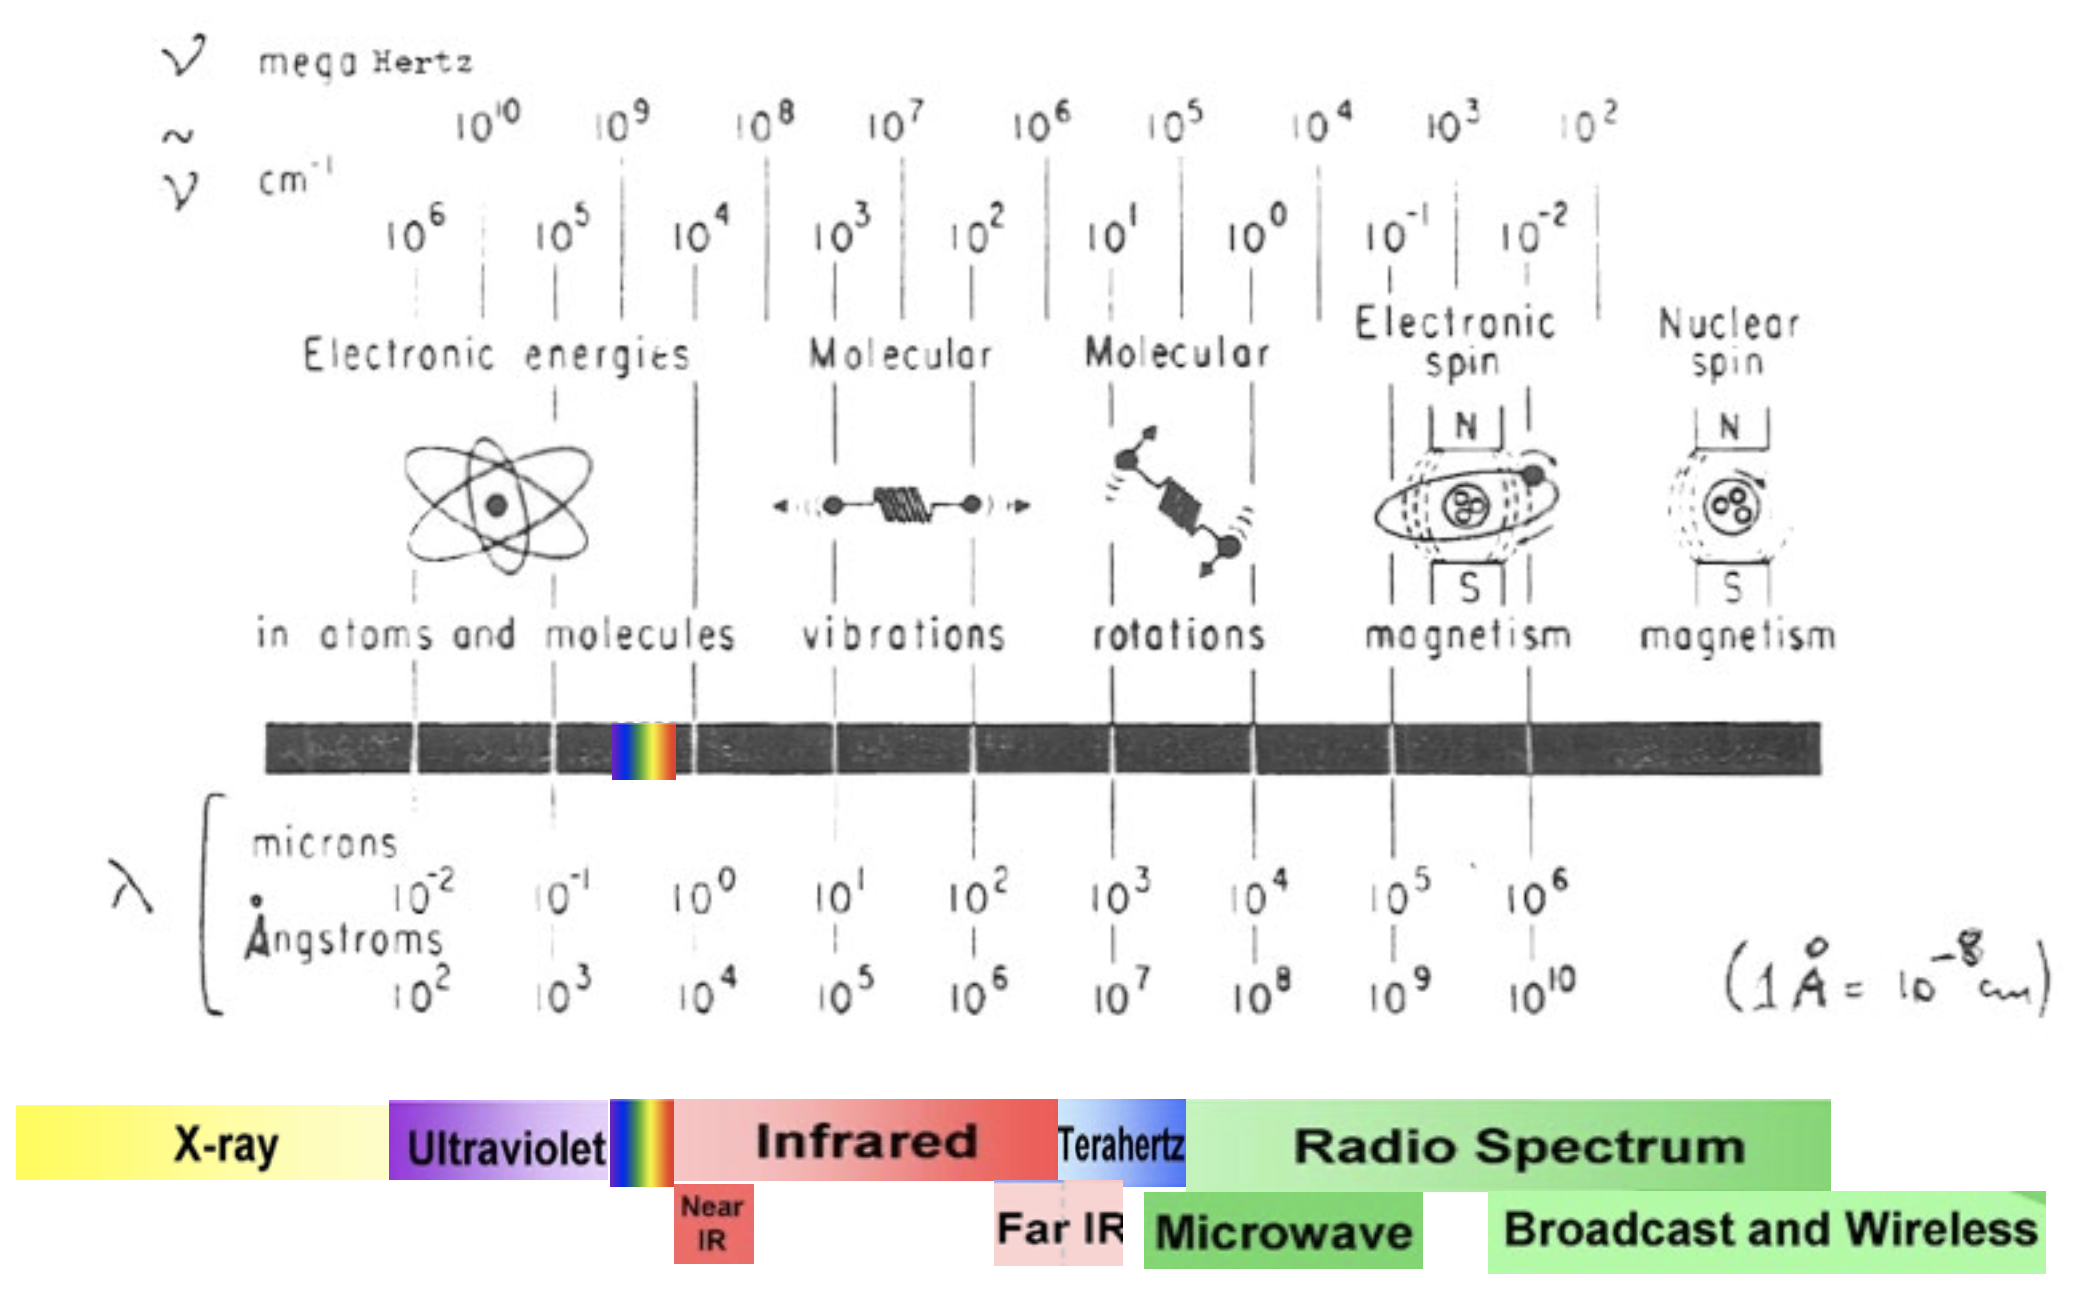
\includegraphics[width=0.68\linewidth]{spectroscopicSpectrum.png}
        \caption{Types of light used by different forms of spectroscopy.}
        \label{fig:spectroscopicSpectrum}
    \end{figure}
    \begin{itemize}
        \item UV/Vis: Electronic absorption (esp. valence electrons).
        \item Infrared: Vibrations.
        \item Microwave: Rotations and crystal lattice vibration.
        \item Radio: NMR.
    \end{itemize}
    \item Goals.
    \begin{itemize}
        \item Understand how light interacts with matter and how you can use this to quantitatively understand your sample (e.g., molecular structure, dynamics, reactivity).
        \item Understand spectroscopy the way you understand other common tools of measurement (like a ruler).
        \item See that spectroscopy is a set of tools that you can put together in different ways to solve the chemical problems that are of interest to you.
    \end{itemize}
    \item A spectrum measures\dots
    \begin{itemize}
        \item The interaction of light with a sample influences the sample and the light.
        \item Two universal steps: Excitation and detection.
        \item Light passes through the sample and then gets characterized on its way out (e.g., absorption, emission, scattering, reflection, dispersion, rotation). We can also characterize a change in the sample (e.g., photothermal, photoelectron and ionization, photochemistry).
        \item In most cases, we characterize how a sample modifies the incident light.
    \end{itemize}
    \item Two common measurements.
    \item \textbf{Absorption}: The attenuation of a light field passing through a sample.
    \begin{itemize}
        \item Photodetectors measure intensity, which is related to the square of the electric field.
    \end{itemize}
    \item \textbf{Emission}: Excitation induces light emission from the sample, typically of a different frequency.
    \item \textbf{Fluorescence}: Emission from singlet states.
    \item \textbf{Phosphoresence}: Emission from triplet states.
    \item \textbf{Raman scattering}: Light taken up shifts the frequency.
    \item The basics of an absorption spectrum.
    \begin{figure}[h!]
        \centering
        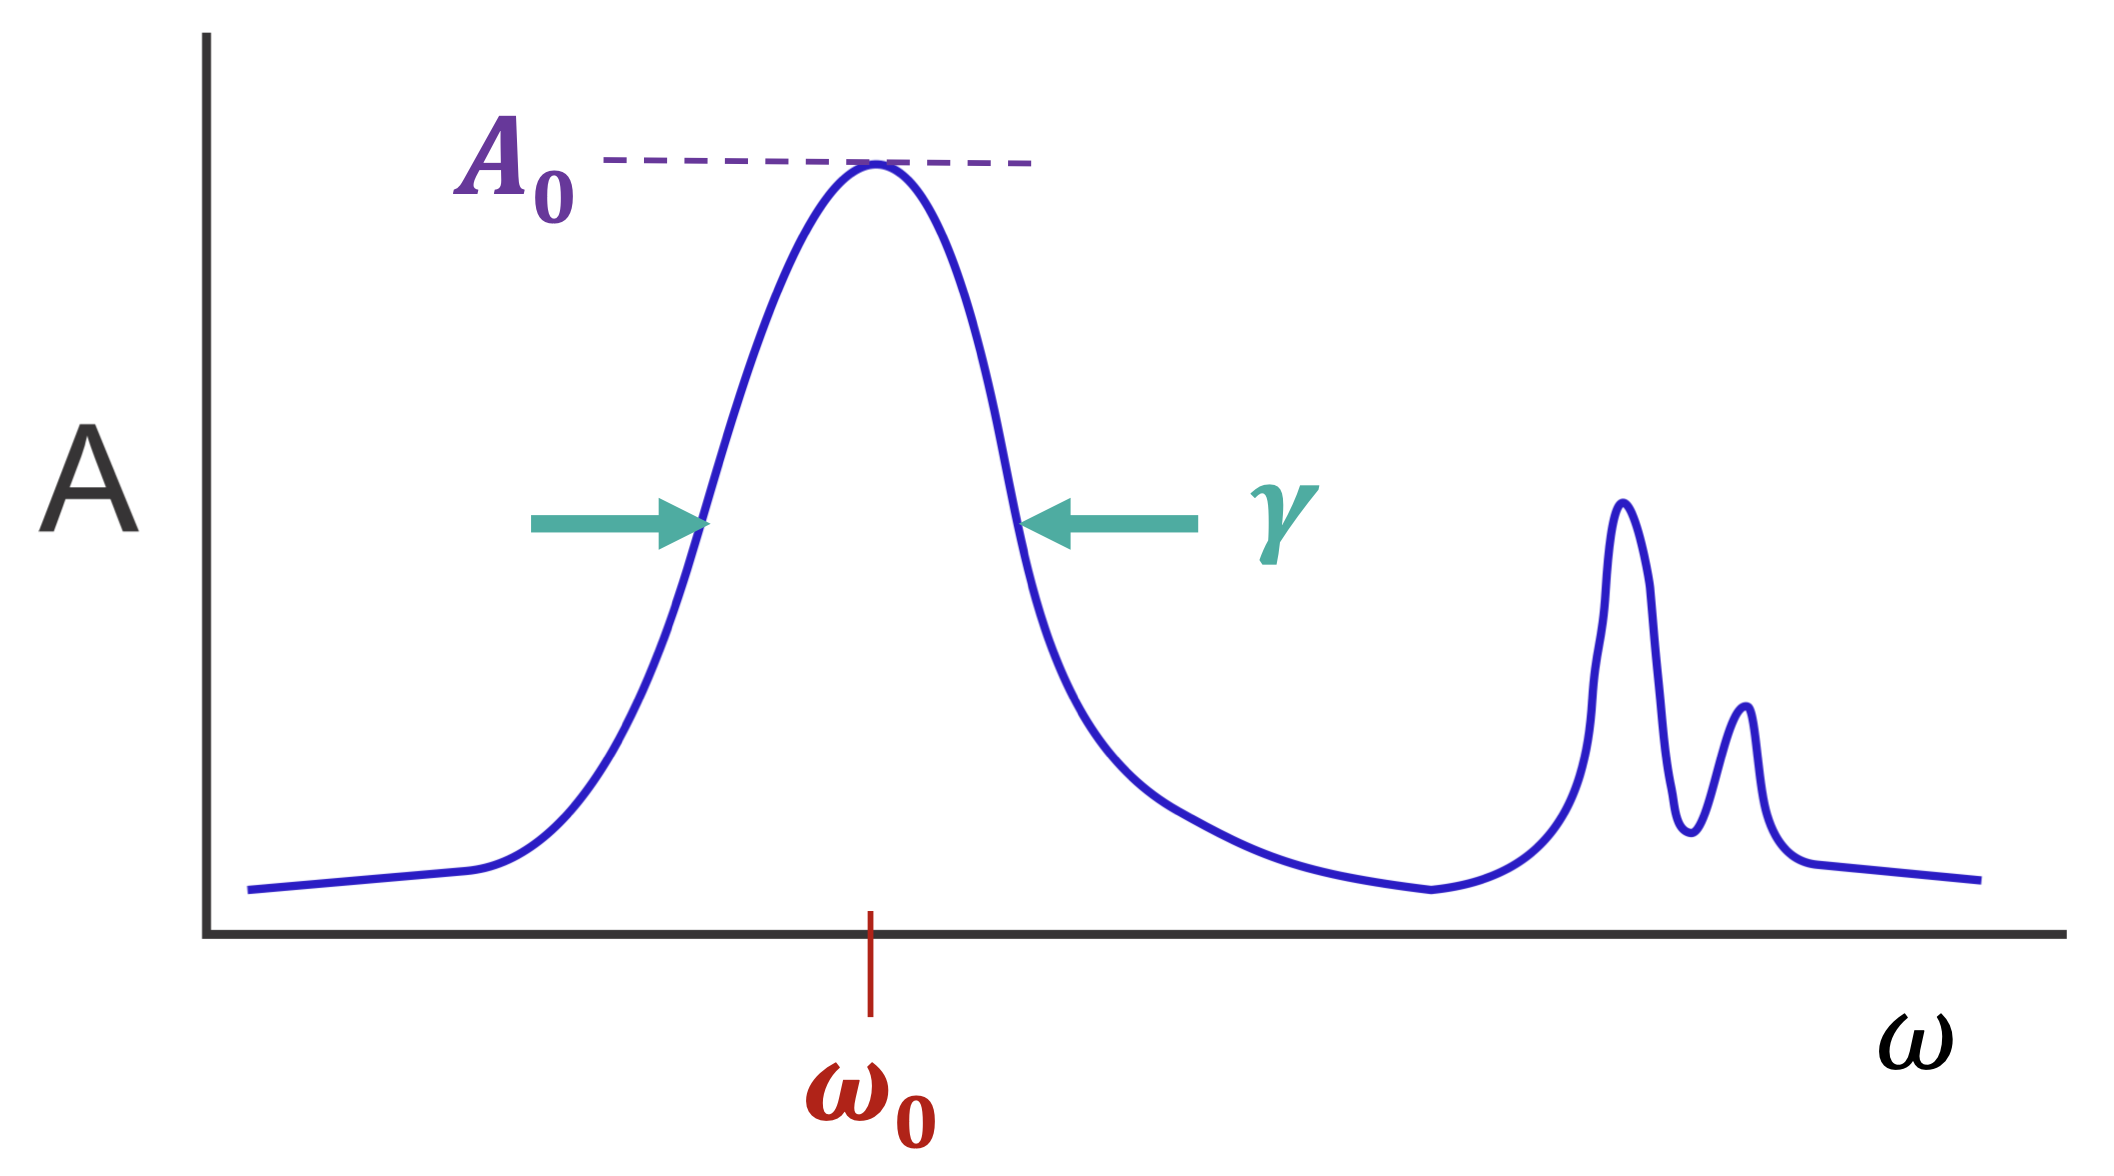
\includegraphics[width=0.35\linewidth]{spectrumFeatures.png}
        \caption{Features of an absorption spectrum.}
        \label{fig:spectrumFeatures}
    \end{figure}
    \begin{itemize}
        \item $x$-axis: Characterizes the input light in terms of frequency (frequency, angular frequency, or wavenumber), wavelength, or energy.
        \item $y$-axis: How the intensity of the light was attenuated at a particular frequency. Look at transmission ($T=I/I_0$) or absorbance ($A=-\log T=\epsilon(\nu)CL$, where $\epsilon$ is the extinction coefficient [unit \si{\liter\per\mole\per\centi\meter}], $C$ is the concentration [unit \si{\molar}], and $L$ is the sample pathlength [unit \si{\centi\meter}]).
        \item Features: Resonance frequency $\omega_0$, peak height $A_0$ or peak area, linewidth $\gamma$ (different frequencies absorbed; gives information on dynamical processes), lineshape (actual functional form of the peak).
    \end{itemize}
    \item How do you measure absorption spectra?
    \begin{itemize}
        \item Measure the change of intensity of light at different frequencies as it passes through a sample.
        \item Two types of spectrometers: Dispersive (common for visible spectrometers) and Fourier transform (more on this later).
    \end{itemize}
    \item \textbf{Dispersive spectrometer}: A spectrometer that has a dispersive element, that is, one that takes white light and spacially spreads the colors of the rainbow.
    \begin{itemize}
        \item Could be a reflection grating, prism, etc.
        \item Measure the white light without the sample, and then with the sample and see what changes. Calculate the transmission, and then absorbance.
    \end{itemize}
    \item That was basic definitions and variables.
    \item This time: We have defined some basic variables for an absorption spectrum.
    \item Next time: Molecular interactions of light. Analyze this mode: Driven electron on a spring.
\end{itemize}




\end{document}